La versione del semaforo trattata in questa sezione del progetto è una versione semplificata del lavoro finale, volta a spiegare il funzionamento del semaforo come progettato. Tale semaforo, infatti, costituisce l'unità fondamentale di questo lavoro ed è poi ripreso successivamente nel progetto finale.

\begin{figure}[H]
    \centering
    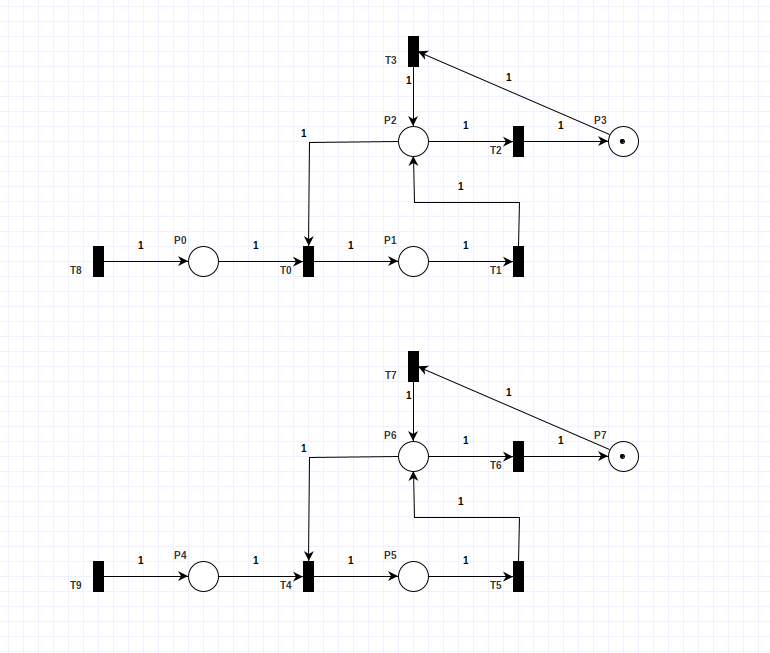
\includegraphics[width=0.6\textwidth]{figure/project_screenshots/semafori.png}
    \caption{Versione base con due semafori}
    \label{fig:semafori}
\end{figure}

In figura \ref{fig:semafori} possiamo vedere una prima bozza di questo progetto. Prendiamo ora in esame solo il semaforo di sopra: il posto P0 rappresenta la fila dei veicoli in attesa di passare, mentre il posto P1 rappresenta un veicolo che attraversa l'incrocio. La transizione T8 a sua volta ha lo scopo di creare un nuovo veicolo da inserire in coda agli altri in P0. I posti P2 e P3, invece, rappresentano una prima struttura di controllo del semaforo: P2 abilita il passaggio, mentre P3 conserva un token bloccando invece il semaforo. Come si può notare, il posto P2 abilita la transizione T0, che permette al veicolo di attraversare l'incrocio. La transizione T1, invece, permette al veicolo di uscire dall'incrocio e di liberare il posto P1 e facendo tornare il token in P2, rendendo il semaforo pronto per un altro attraversamento o per passare al rosso (P3).

Tuttavia, tale versione presenta alcuni importanti difetti che non è possibile ignorare: allo stato attuale i due semafori possono lavorare in maniera indipendente, rendendo possibili scenari pericolosi quali l'attraversamento contemporanreo di due veicoli. A tal scopo. quindi, sono state implementate due GMEC: 

\begin{itemize}
    \item \textbf{GMEC 1}: solo un semaforo alla volta può essere verde:
    \begin{equation}
        M(P_{2}) + M(P_{6}) \leq 1
    \end{equation}

    \item \textbf{GMEC 2}: non è possibile che due veicoli si incrocino:
    \begin{equation}
        M(P_{1}) + M(P_{5}) \leq 1
    \end{equation}
\end{itemize}

\begin{figure}[H]
    \centering
    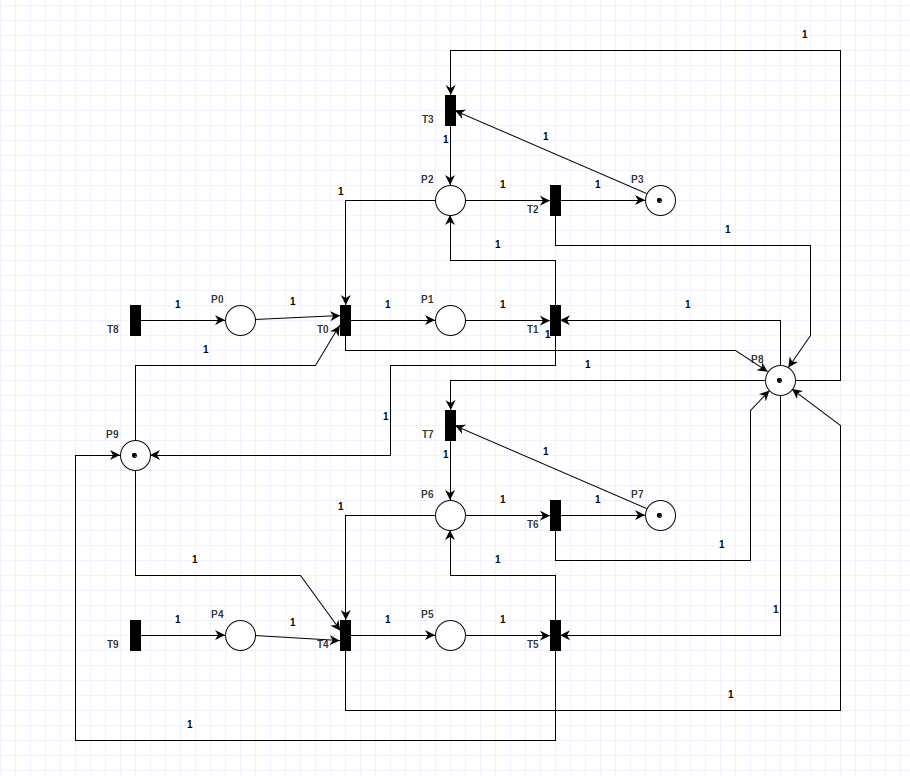
\includegraphics[width=0.6\textwidth]{figure/project_screenshots/semafori_con_controllo.png}
    \caption{Versione con GMEC}
    \label{fig:semafori_gmec}
\end{figure}

Grazie a questi due vincoli, il semaforo diventa come quanto mostrato in figura \ref{fig:semafori_gmec}. In questo modo, quindi, è possibile garantire un attraversamento stradale sicuro e ordinato dell'incrocio.